\documentclass[letterpaper, 10 pt, conference]{ieeeconf}
%\documentclass[10pt,a4paper]{article}
\IEEEoverridecommandlockouts % This command is only needed if you want to use the \thanks command

\overrideIEEEmargins % Needed to meet printer requirements.

\usepackage[latin1]{inputenc}
\usepackage{amsmath}
%\usepackage{amsthm}
\usepackage{amsfonts}
\usepackage{amssymb}
\usepackage{mathtools}
\usepackage{graphicx}
\usepackage{color}
%\usepackage{hyperref}

% theorem environment
\newtheorem{prop}{Proposition}[section]
\newtheorem{theorem}{Theorem}[section]
\newtheorem{prop2}{Proposition}
\newtheorem{lem}{Lemma}
\newtheorem{ex}{Example}

% For algorithms
\usepackage{algorithm}
\usepackage{algorithmic}

% custom commands
\newcommand{\boldvec}[1]{\boldsymbol{\mathrm{#1}}}
\let\vec\boldvec
\newcommand\at[2]{\left.#1\right|_{#2}} % the at differential sign
\newcommand\scalemath[2]{\scalebox{#1}{\mbox{\ensuremath{\displaystyle #2}}}} % scaling matrices

%% custom macros

% % % % % % % % Notation for robot % % % % % % %
\newcommand{\todo}{\textcolor{red}{TODO}} % TODO!
\newcommand{\kin}{\mathcal{K}} % used to denote forward kinematics
\newcommand{\invKin}{\mathcal{K}^{-1}} % used to denote inverse kinematics

\newcommand{\joint}{\vec{q}} % used to denote robot state in joint space
\newcommand{\state}{\vec{y}} % denotes the generalized coordinates - joint angles and angular velocities
\newcommand{\error}{\vec{e}} % difference between state and reference
\newcommand{\traj}{\vec{r}} % used to denote the points on the trajectory to be tracked

\newcommand{\dynamics}{\vec{f}}
\newcommand{\dynamicsNominal}{\dynamics_{\mathrm{nom}}}
\newcommand{\dist}{\vec{\epsilon}} % denotes the disturbances acting on the rigid body dynamics
\newcommand{\sysInput}{\vec{u}} % used to denote the system inputs
\newcommand{\trjInput}{\sysInput_{\mathrm{IDM}}} % denotes the inputs on the trajectory (calculated using IDM)

\newcommand{\policy}{\vec{\pi}}
\newcommand{\ValueFunction}{J}
\newcommand{\episode}{k} % used for episode number
\newcommand{\totalTime}{T} % total time duration 
\newcommand{\numSteps}{N} % total number of time steps
\newcommand{\threshold}{\epsilon}
\newcommand{\alg}{\emph{ptt}} % probabilistic table tennis
\newcommand{\dataset}{\mathcal{D}}

% % % % % % % % Table tennis notation % % % % % %
\newcommand{\ballFull}{\vec{x}_{B}} % ball cartesian state
\newcommand{\ball}{\vec{b}} % ball positions
\newcommand{\ballDynamics}{\vec{F}} % ball dynamics
\newcommand{\drag}{C} % drag
\newcommand{\gravity}{g}
\newcommand{\bounce}{\vec{E}} 
\newcommand{\contact}{\vec{C}} % contact model
\newcommand{\racket}{\vec{r}} % racket positions
\newcommand{\racketRadius}{r} % racket radius
\newcommand{\orient}{\vec{o}} % racket orientations
\newcommand{\normal}{\vec{n}} % racket normal
\newcommand{\robot}{\vec{x}_{R}} % racket state involving pos,vel and orient
\newcommand{\court}{\mathcal{T}} % opponents court
\newcommand{\net}{\mathcal{N}} % net
\newcommand{\wall}{\mathcal{W}} % wall

% % % % % % % % Probability notation % % % % % % %
\newcommand{\prob}{\mathbb{P}} % probability
\newcommand{\landTime}{\tau} % random variable
\newcommand{\landDist}{p(\tau)} % distribution of landing time
\newcommand{\hitTime}{\nu} % hitting time
\newcommand{\hitDist}{p(\nu)} % distribution of hitting time


% Set the paths where all figures are taken from:
\graphicspath{{Pictures/}}
\mathtoolsset{showonlyrefs} 
\newcommand{\includesvg}[1]{%
% \executeiffilenewer{#1.svg}{#1.pdf}%
% {inkscape -z -D --file=#1.svg %
% --export-pdf=#1.pdf --export-latex}%
 \input{#1.pdf_tex}%
}

\author{Okan Ko\c c$^{1}$, Guilherme Maeda$^{2}$, Jan Peters$^{1,2}$% <-this % stops a space 
\\
{\tt\small \{okan.koc, jan.peters\}@tuebingen.mpg.de}%
\thanks{$^{1}$Max Planck Institute for Intelligent Systems,
        Spemannstr. 38, 72076 Tuebingen, Germany}
\thanks{$^{2}$Technische Universitaet Darmstadt, FG Intelligente Autonome Systeme
        Hochschulstr. 10, 64289 Darmstadt, Germany}
}
\title{A New Performance Criterion in Robotic Table Tennis}

\begin{document}

\maketitle
\thispagestyle{empty}
\pagestyle{empty}

%%%%%%%%%%%%%%%%%%%%%%%%%%%%%%%%%%%%%%%%%%%%%%%%%%%%%%%%%%%%%%%%%%%%%%%%%%%
\begin{abstract}

In highly dynamics tasks that involve moving targets, planning is necessary to figure out when, where and how to intercept the target. In robotic table tennis in particular, conventional planning algorithms often rely on the virtual hitting plane hypothesis to construct robot striking trajectories. These algorithms however are vulnerable to modeling and execution errors. %For example, the trajectories they generate are not robust to uncertainty in ball position and velocity at hitting time. 
Moreover, they do not take advantage of the inherent task redundancy when planning trajectories. In this paper, we address these two issues by introducing a new performance criterion for robotic table tennis. We use an optimal control approach to construct a novel inverse-kinematics algorithm that does not involve a fixed hitting plane. Furthermore, by augmenting our cost functional with a probabilistic final-cost we incorporate the uncertainties in modeling, estimation and execution as well as task redundancy. Our algorithm returns the balls with a higher probability to the opponents court in two and three dimensional table tennis with different robot models when compared with a state of the art planning approach. 

% better term for task redundancy?
% certainty-equivalent, cautious


\end{abstract}

%%%%%%%%%%%%%%%%%%%%%%%%%%%%%%%%%%%%%%%%%%%%%%%%%%%%%%%%%%%%%%%%%%%%%%%%%%%

%\section{INTRODUCTION}\label{introduction}

% fill missing citations

Most reaching tasks in control and robotics can be phrased as \emph{tracking} problems, where the dynamical system needs to follow a certain predefined trajectory in order to reach the goal state. Robotic table tennis in particular~\cite{Muelling13} consists of planning, generating and executing a series of such (episodic) single stroke trajectories. These trajectories need to be followed very closely with motor commands in practice, in order to return the ball to the goal position. 

% maybe cite Jens' review paper
There have been many attempts in the reinforcement learning (RL)~\cite{Sutton98} and control literature to learn robotic tasks directly. Value function based methods take advantage of duality to solve the Bellman's equation but suffer from the initial bias or representation in estimating the value function and do not scale well to high dimensions. Policy search based RL methods (e.g.,~\cite{Kober08}, \cite{Peter10}, \cite{Theodorou10}, \cite{Deisenroth11}) directly solve the Bellman's equation in a parameterized policy space and can be more effective in practice~\cite{Kober13}. 

Dynamic Movement Primitives (DMP) are a kind of kinematic policy representation that leverages the dynamical systems approach to modify the spring dynamics with a forcing term that enables it to mimic an executed trajectory. They include an internal phase or clock that ensures the convergence of the movement primitive to a goal state~\cite{Ijspeert13}, \cite{Schaal07}. DMPs do not suffer from the curse of dimensionality as the number of parameters (weights) grow linearly with dimension. However, approximation and control errors in robotic platforms make the application of DMPs less useful in practice. Small changes to DMPs can often make them more useful.

Motor primitives can be modulated in different ways to adapt to unforeseen events or to ensure the optimal execution of required tasks. They work particularly well with episodic policy search methods that modify the weights of the forcing term based on the rewards received in every episode. By adapting the DMP that was initialized with imitation learning e.g., with kinesthetic teach-in~\cite{Muelling13}, RL approaches are able to achieve complex robotic tasks, such as ball-in-a-cup~\cite{Kober09}. However model-free methods (e.g., \cite{Kober08}, \cite{Peter10}) require many iterations to converge, whereas more data-efficient approaches such as~\cite{Deisenroth11} suffer from computational runtime difficulties and cannot be implemented in real-time robotics tasks. Optimality of the converged policy cannot be guaranteed by these methods.
% maybe mention reference trajectory?
% model-free ? PILCO claims to be 'model-based', yet it learns from scratch. It only 'learns' a model, but it is unbiased.

% inaccurate ?
Inspired by the successes (and failures) of these previous approaches, the research question that we tackle in this article consists of the following:
%
\begin{itemize}
\item How can we execute optimally hitting movement primitives either in table tennis or a similar reaching task e.g., putting in golf.
%
\item More specifically, when we have modelling inaccuracies, how should we modify a DMP $\dmp(t)$ such that the robot executes a desired hitting motion?
\end{itemize}
%
\begin{figure}[b!]
\center
\includegraphics[scale=0.4]{robot1.png}			
\caption{Robotic table tennis setup with the ball-launcher throwing balls to the robot. In order to hit the ball to a desired position on the opponent's court, we give the robot reference trajectories that facilitate the right striking motion. We can teach the robot such trajectories via kinesthetic teach-in.}
\label{robot}
\end{figure}
%
% maybe include P. Abbeel's work on inaccurate models
\noindent We believe that learning in robotics tasks can be performed much more efficiently by taking advantage of existing imperfect models and reference trajectories. % optimality issues can be alleviated with given reference trajectories. 

Iterative Learning Control (ILC) is a fundamental approach in control theory developed to track (time-varying) reference trajectories. It has been used successfully to follow trajectories under unknown repeating disturbances and model mismatch \cite{Bristow06}. In ILC, control inputs are adjusted at each episode in a feedforward fashion. The goal is to drive the deviations from the trajectory to zero. 
% or equivalently references

In this article, we combine Iterative Learning Control with movement primitives by using ILC as a learning method to adapt the weights of the DMPs. This way we ensure a safe, reliant and robust way to track reference trajectories, with important applications in optimally hitting and striking motions. As opposed to model-free policy search approaches, we make full use of the known, albeit inexact, robot dynamics and inverse dynamics models, which helps us to quickly achieve the desired performance requirements. We validate the performance of the approach in two hitting tasks, and compare with existing episodic-RL approaches.
% nominal model instead of known, albeit inexact?

Our contributions can be summarized as follows: we form a link between the ILC literature and the movement primitives by systematically formulating an iterative update of the DMP weights. We form a coherent learning framework and present new motor primitive update laws. These are studied in detail and the implemented ILC algorithm~$\alg$ is shown to perform better than existing RL approaches in two hitting tasks, putting and table tennis.

In Section~\ref{relatedWork} we mention related work, especially the state of the art approaches in hitting and reaching tasks. In Section~\ref{problemStatement} we state the problem and introduce motor primitive update laws, relating them to the existing optimization-based ILC approaches. We formulate one of these update laws, called $\alg$, in algorithmic form in Section~\ref{algorithm}. In Section~\ref{experiments} we evaluate $\alg$ in two robotic reaching tasks: putting motion in golf and the striking motions in table tennis. We show that the method outperforms the state-of-the-art RL-based approaches \emph{REPS} and \emph{PI$^{2}$}. Finally in Section~\ref{conclusion} we discuss the strengths and weaknesses of our method and conclude with brief mentions of promising future research directions.

\subsection{Related Work}\label{relatedWork}

% mention the ILC paper of Peter Abbeel
Dynamic movement primitives belong to the class of movement primitives~\cite{Flash85}. Movement primitives are a kinematics-based approach to keep the learning tasks in high-dimensional tasks, such as in humonoid robotics, tractable. Like the options framework in Markov Decision Processes, they aim at reducing the curse of dimensionality in complex human-like robotics tasks. The first dynamical systems based formulation of movement primitives appeared in~\cite{Ijspeert02}. A good review with alternative and variant formulations is given in~\cite{Ijspeert13}.

% Policy search methods
One of the first examples of policy search based methods that modify the parameters of movement primitives is the \emph{POWER} algorithm~\cite{Kober08}. \emph{PI$^{2}$} algorithm has a very similar implementation in~\cite{Theodorou10} and episodic-\emph{REPS}~\cite{Peter10} is actually equivalent to \emph{POWER}.

Iterative Learning Control started out in the 1980s with the work of Arimoto et al.~\cite{Arimoto84} as one of the first to define the genre with the PD-type update law. See~\cite{Bristow06} and \cite{Moore99} for reviews. Monotonic convergence and stability guarantees are of central importance for the practical usefulness of ILC algorithms. They are shown for example in~\cite{Bristow06}, \cite{Norrloef02}, \cite{Longman2000}.

% ILC work - mention Angela's work
As an example of a more sophisticated method than the PD-type update laws, Schoellig et al.~\cite{Schoellig12} applied a Kalman-filter based convex optimization rule in the framework of ILC and showed its performance in quadrocopter flight. An EM-based update law was given in~\cite{Berg10} where an impressive application of ILC to a robotic surgical task was presented.
% This work however lacks any guarantees of monotonic convergence

% DMPs using Iterative Learning Control
DMPs have been also combined in a bimanual robotics task with ILC~\cite{Gams13} where force feedback is used to enable compliant interaction with objects in an unknown environment. ILC is here used to learn a coupling term between the two arm trajectories. To the best of our knowledge, ILC has not been used so far to modify the weights of the movement primitives.
% used to modulate the DMP and learn ...

\subsection{Problem Statement}\label{problemStatement}

The goal in trajectory tracking is to track a given reference $\traj(t), \ 0 \leq t \leq T \ $, in state space $\state \in S \subset \mathbb{R}^{n}$ by applying the control inputs $\sysInput(t)$. The reference trajectory in our case enables the \emph{optimal} execution of hitting and striking motions, e.g., forehand and backhand strikes in (table) tennis. We assume that such optimal trajectories are available to us, either through kinesthetic teach-in or computed recursively.
% talk about feasibility.
% reference needed? Dynamic programming?

% subsubsection entitled 'modelling assumptions'?
% talk of model-free regression update of DMP there maybe?
Consider the nonlinear robot dynamics of the form
%
\begin{equation}
\begin{aligned}
\ddot{\joint} &= \dynamics(\joint,\dot{\joint},\sysInput), \\
\ddot{\joint} &= \vec{M}^{-1}(\joint)\{ \vec{\tau}(\sysInput) - \vec{C}(\joint,\dot{\joint})\dot{\joint} - \vec{G}(\joint)\} + \dist(\joint,\dot{\joint}),\\
\end{aligned}
\label{dynamics}
\end{equation}
%
\noindent where on the right hand side are the terms due to the rigid body dynamics model and $\dist(\joint,\dot{\joint})$ are the (unmodeled) disturbances that act on the robot, such as viscous friction, stiction, etc. This system can be linearized around a given joint space trajectory $\traj(t), \ 0 \leq t \leq T$ with nominal inputs $\trjInput(t)$ calculated using the inverse dynamics model. We then obtain the following linear time varying (LTV) representation
%
\begin{equation}
\begin{aligned}
\dot{\error} = \vec{A}^{c}(t)\error(t) + \vec{B}^{c}(t)\linInput(t) + \linDist(t,\sysInput),
\end{aligned}
\label{LTV}
\end{equation}
%
\noindent where the state error is denoted as $\error(t) = \state(t) - \traj(t)$, the joint angles and velocities are $\state = [\joint,\dot{\joint}]^{\mathrm{T}}$, $\linInput(t) = \sysInput(t) - \trjInput(t)$ and the continuous time varying matrices are
%
\begin{equation}
\begin{aligned}
\vec{A}^{c}(t) &= \at{\frac{\partial{\dynamics}}{\partial{\state}}}{(\traj(t),\trjInput(t))}, \\
\vec{B}^{c}(t) &= \at{\frac{\partial{\dynamics}}{\partial{\sysInput}}}{(\traj(t),\trjInput(t))}.
\end{aligned}
\label{LTVmatrices}
\end{equation}
%
% what about estimation errors, i.e. sensor errors ...
\noindent In the error dynamics \eqref{LTV} the additional term $\linDist(t,\sysInput)$ accounts for the disturbances and the effects of the linearization. We can discretize (\ref{LTV}-\ref{LTVmatrices}) with step size $\delta$, $N = T/\delta$ and step index $j = 1, \ldots, N$ to get the following discrete linear system
%
\begin{equation}
\begin{aligned}
\error_{j+1} = \vec{A}_j\error_j + \vec{B}_j\linInput_j + \linDist_j(\sysInput_1, \ldots, \sysInput_j),
\end{aligned}
\label{discreteLTV}
\end{equation}
%
\noindent where the matrices $\vec{A}, \vec{B}$ are the discretizations of \eqref{LTVmatrices}. Conventional ILC algorithms learn to compensate for the errors by iterating the control inputs $\sysInput$ with an update law.
%\section{Iterative Learning Control with Movement Primitives}\label{method}

In a complex task such as robot table tennis, one often needs to consider an extension of the standard trajectory tracking task. Based on the varying initial positions and velocities of the robot arm and the trajectory of the incoming ball, in each table tennis stroke the robot arm needs to track different trajectories that start from different initial conditions and end with different goal states of the arm. Moreover these trajectories need to be scaled in time to intercept the ball. Dynamic Movement Primitives (DMP) are especially useful for representing such a variety of movement patterns.
% reference needed? revise.

%Sometimes for safety reasons, for instance when interacting with external objects or under unforeseen perturbations \cite{Schaal07}, a \emph{low-gain} feedback law operating on the inputs may be fine-tuned to be compliant. As another practical restriction, one may not even be allowed to modify the low-level controller of the industrial robot \cite{Longman2000}. In such cases, it is not possible to modify the input signals $\sysInput$ directly. Instead one can modify the reference trajectories that are provided to the low-level controllers. It can be shown that this is an equivalent approach to modifying the feedforward control inputs \cite{Bristow06}.

Based on these considerations, in this paper we focus on learning to track DMPs $\dmp(t) = [\joint_{\text{des}}(t),\dot{\joint}_{\text{des}}(t)]^{\mathrm{T}}$. An initial DMP might be constructed out of a given demonstration or an optimal reference trajectory $\traj(t)$ using regression techniques \cite{Ijspeert13}. Representing a reference trajectory with movement primitives has some benefits: nonsmooth parts of the trajectory can be filtered, the evolution of desired states can be coupled with errors to ensure safety, time and scaling invariance of the differential equations can be used to adapt the trajectory to task changes in time as well as in space. %Robustness to initial joint position and velocity changes 

\subsection{Movement Primitive Formulation}
The dynamic movement primitive equations~\cite{Kober08} can be written as a weakly nonlinear system 
%
\begin{equation}
\begin{aligned}
\dot{\dmp} &= \begin{bmatrix}
   \dot{\dmp}_1 \\
   \dot{\dmp}_2
 \end{bmatrix} = \tau \begin{bmatrix}
     \dmp_2  \\
     \alpha_{g} (\beta_{g}(\goal - \dmp_1) - \dmp_2) +  \vec{\phi}(\phase)\weights
  \end{bmatrix}
\label{dmp},
\end{aligned}
\end{equation}
%
\noindent where the phase $\phase$ evolves according to
%
\begin{equation}
\dot{\phase} = -\tau\alpha_{\phase}\phase.
\label{phase}
\end{equation}
%
\noindent The constants $\tau$ and $\alpha_{\phase}$ determine the scaling and settling time respectively. 

The dynamical system \eqref{dmp} describes the motion of each of the desired joint states along a particular path in joint space. The forcing terms $\force = \vec{\phi}(\phase)\weights$ determine this path by warping the motion of the spring dynamics. The weights $\weights$ are obtained from regression using demonstration data. The spring constants $\alpha_{g}$ and $\beta_{g}$ ensure that starting from any initial position and velocity $\dmp_0$ the DMP converges to the goal state $\goal := \dmp_T = \traj_T$ and are usually chosen such that the dynamical system is critically damped.

% mention Jens' and Katharina's extension for hitting DMPs with desired velocity

% a figure showing convergence from different starting conditions needed here

\subsection{Derivation of ILC Updates}

Most ILC update laws can be put in the following form

\begin{equation}
\begin{aligned}
\sysInput_{k+1} = \qmatrix(\sysInput_{k} - \lmatrix\error_{k}).
\end{aligned}
\label{ILCupdateForm}
\end{equation}

\noindent Model based ILC can be cast in this form by stacking the model matrices in \eqref{discreteLTV} together to get the following lifted-vector representation \cite{Bristow06}, \cite{Schoellig12}

\begin{equation}
\begin{aligned}
\error_L &= \vec{F}\sysInput_L + \linDist_L, \\
\end{aligned}
\label{liftedLTV}
\end{equation}

\noindent where the submatrices of $\vec{F}$ are

\begin{equation*}
\begin{aligned}
\vec{F}_{(i,j)} &= \left \{
\begin{array}{cc}
\vec{A}_{i-1}\ldots \vec{A}_j \vec{B}_{j-1}, & j < i, \\ 
\vec{B}_{j-1}, & j = i, \\
\vec{0}, & j > i. 
\end{array} \right.
\end{aligned}
\end{equation*}

\noindent Using this \emph{input-to-output matrix} $\vec{F}$ we can analyze the effects of the feedforward inputs $\sysInput_L = [\linInput_1, \linInput_2, \ldots, \linInput_{\numSteps}]^{\mathrm{T}}$ on the errors $\error_L = [\error(1),\error(2),\ldots,\error(\numSteps)]^{\mathrm{T}}$ and compensate for the disturbances $\linDist_L$ with ILC.

%\noindent If the disturbances are repeating every iteration, i.e. $\frac{\partial{\linDist_L}}{\partial{\sysInput_L}} = 0$, using \eqref{liftedLTV},

\subsubsection{Lagrange form} The quadratic cost functional as the optimality criterion

\begin{equation}
\begin{aligned}
\ValueFunction(\state_0) &= \int_{0}^{T} \error^{\mathrm{T}}\vec{Q}\error + \linInput^{\mathrm{T}}\vec{R}\linInput \ \mathrm{d}t + \error_{T}^{\mathrm{T}}\vec{Q}_{T}\error_{T},
\end{aligned}
\label{cost}
\end{equation}

\noindent can be equally discretized and stacked in lifted vector form

\begin{equation}
\begin{aligned}
\ValueFunction_L &= \error_L^{\mathrm{T}}\vec{Q}_L\error_L + \sysInput_L^{\mathrm{T}}\vec{R}_L\sysInput_L,
\end{aligned}
\label{costFunctional}
\end{equation}

\noindent where $\vec{Q}_L \in \mathbb{R}^{2Nn \times 2Nn}$ (similarly for $\vec{R}_L$) is of the following form
%
\begin{equation*}
\begin{aligned}
 \vec{Q}_L &= 
 \begin{bmatrix}
  \vec{Q} & \vec{0} & \cdots & \vec{0} \\
  \vec{0} & \vec{Q} & \cdots & \vec{0} \\
  \vdots  & \vdots  & \ddots & \vdots  \\
  \vec{0} & \vec{0} & \cdots & \vec{Q}_T
 \end{bmatrix}.
\end{aligned}
\end{equation*}

\noindent Using Gauss-Newton we can optimize iteratively for $\sysInput_L$

\begin{equation}
\begin{aligned}
\sysInput_{k+1} &= \sysInput_k - \Big(\frac{\partial^{2}\ValueFunction_L}{\partial\sysInput^{2}_L}\Big)^{-1}\at{\frac{\partial{\ValueFunction_L}}{\partial{\sysInput_L}}}{\sysInput_k} \\
\frac{\partial^{2}\ValueFunction_L}{\partial\sysInput^{2}_L} &= \frac{\partial}{\partial\sysInput_L}\{F^{\mathrm{T}}Q_L\error_L\} = F^{\mathrm{T}}Q_LF \\
\sysInput_{k+1} &= \sysInput_k - \beta_kF^{\dagger}\error_k
\end{aligned}
\label{ILCnewtonsMethod}
\end{equation}

\noindent ILC update law can be related to Newton's method if we consider the Hessian of the cost functional \eqref{cost2}
%
\begin{equation}
\begin{aligned}
\weights_{k+1} &= \weights_k - \beta_k\Big(\frac{\partial^{2}\ValueFunction}{\partial\weights^{2}}\Big)^{-1}\at{\frac{\partial{\ValueFunction}}{\partial{\weights}}}{\weights_k}, \\
\frac{\partial^{2}\ValueFunction}{\partial\weights^{2}} &= \frac{\partial}{\partial\weights}\{\vec{F}_{w}^{\mathrm{T}}\vec{Q}_L\error_L + \vec{R}_w\weights\} = \vec{F}_{w}^{\mathrm{T}}\vec{Q}_L\vec{F}_{w} + \vec{R}_{\weights}, \\
\weights_{k+1} &= \qmatrix\weights_k - \beta_k(\vec{F}_{w}^{\mathrm{T}}\vec{Q}_L\vec{F}_{w} + \vec{R}_{w})^{-1}\vec{F}_{w}^{\mathrm{T}}\vec{Q}_L\error_k,
\end{aligned}
\label{ILCWeightsNewtonsMethod}
\end{equation}
%
\noindent where the filtering matrix is $\qmatrix = \beta_k(\vec{F}_{w}^{\mathrm{T}}\vec{Q}_L\vec{F}_{w} + \vec{R}_{w})^{-1}\vec{R}_{w}$. 

Note the connection of \eqref{ILCWeightsNewtonsMethod} to plant inversion methods~\cite{Bristow06}: taking $\vec{Q}_L = \vec{I}, \vec{R}_{w} = \vec{0}, \beta = 1,$ \eqref{ILCWeightsNewtonsMethod} becomes
%
\begin{equation}
\begin{aligned}
\weights_{k+1} &= \weights_k - \vec{F}_{w}^{\dagger}\error_k.
\end{aligned}
\label{ILCPlantInversion}
\end{equation}
%
% However this can be very unstable in practice, especially in nonminimum phase systems. Having a small, but nonzero weighting matrix R makes it much more stable.
%
\noindent Notice also the connection of \eqref{ILCRegression} with the online regression methods performed on the DMP weights \cite{Ijspeert13}. We can rewrite \eqref{ILCWeightsNewtonsMethod} as
%
\begin{equation}
\begin{aligned}
\weights_{k+1} &= \weights_k - \beta_k(\vec{\Psi}^{\mathrm{T}}\vec{W}\vec{\Psi} + \vec{R}_{w})^{-1}\vec{\Psi}^{\mathrm{T}}\vec{W}\error_k, \\
\vec{\Psi} &= \begin{bmatrix}
  \basis_1^{T} & \basis_2^{T} & \ldots & \basis_N^{T}
 \end{bmatrix}^{T}.
\end{aligned}
\label{ILCRegression}
\end{equation}
%
%
% online regression methods? are they discussed in the given reference?
In model-free approaches the weighting matrix $\vec{W}(t)$ is taken as the identity matrix. In our case the model-based assumptions of our approach appear in the form of a nondiagonal covariance matrix. We perform generalized least-squares regression by taking advantage of the linearized model in~\eqref{fullTransition} to form the right correlations between states. Compared with the \emph{credit-assignment} issues of RL algorithms, we see that ILC, equipped with our linearized models, offers us a more principled way to assign errors to the weights of the movement primitives.

\subsubsection{Mayer form}

\subsection{Iterative Learning Control for Movement Primitives}\label{ilcOnDMP} 

For the linearization of the robot dynamics \eqref{dynamics} under a given linear feedback law $\linInput(t) = -\vec{K}(t)(\state - \dmp)$ we consider the addition of the movement primitive dynamics to \eqref{LTV} 
%
\begin{equation}
\begin{aligned}
\dot{\fullvec} &= \vec{A}_{\fullvec}\fullvec(t) + \vec{B}_{\fullvec} \weights + \linDist(t,\weights),
\label{fullTransition}
\end{aligned}
\end{equation}
%
\noindent where for the enlarged vector $\fullvec = [\error,\dmp]^{\mathrm{T}}$ the transition matrices are 
%
\begin{IEEEeqnarray}{rCl}
%\footnotesize
\arraycolsep=3pt
\medmuskip = 1mu
\begin{aligned}
 \vec{A}_{\fullvec} &= \begin{bmatrix}
  \vec{A}(t) - \vec{B}(t)\vec{K}(t) & \vec{B}(t)\vec{K}(t) \\
  \vec{0} & \vec{A}_s
 \end{bmatrix}, \\
 \vec{B}_{\fullvec} &= \begin{bmatrix}
    \vec{0} \\
    \vec{\basis}(\phase)
   \end{bmatrix}. 
\end{aligned}
\label{fullMatrices}
\end{IEEEeqnarray}
%
\noindent The system matrices $\vec{A}$ and $\vec{B}$ ensure the coupling of the DMP to the states. 
%Reference trajectory $\traj(t)$ moves with a given velocity $\nu(t)$.

By detaching the reference trajectory $\traj(t)$ from the feedback law and hence from the dynamics \eqref{fullTransition} we can consider applying ILC techniques to the movement primitives $\dmp$. If we introduce the following cost functional as our optimality criterion
%
% We don't need the continous form!
%
\begin{IEEEeqnarray}{rCl}
\begin{aligned}
J(\weights) =& \int_{0}^{T} \error^{\mathrm{T}}\vec{Q}\error + \weights^{\mathrm{T}}\vec{R}_w \weights \ \mathrm{d}t \ \scalebox{0.9}[1]{\( + \)} \, (\state_T\scalebox{0.85}[1.0]{\( - \)}\goal)^{\mathrm{T}}\vec{Q}_{T}(\state_T\scalebox{0.85}[1.0]{\( - \)}\goal),
\end{aligned}
\label{cost2}
\end{IEEEeqnarray}
%
\noindent we can apply a weight-update form of the ILC update law~\cite{Bristow06}
%
\begin{equation}
\begin{aligned}
\weights_{k+1} = \qmatrix(\weights_{k} - \lmatrix\error_{k}),
\end{aligned}
\label{ILCupdateFormWeights}
\end{equation}
%
\noindent to minimize \eqref{cost2}. The index $k = 0, 1, \ldots$ denotes the iteration number. The matrices $\qmatrix$ and $\lmatrix$ are the filtering and learning matrices respectively~\cite{Bristow06}. They modulate the dependency between the inputs $\weights$ and the errors $\error$. Depending on these two matrices, the ILC update law \eqref{ILCupdateFormWeights} can be designed to be noncausal (i.e. predictive) and iteration-dependent. In order to reach the weight update law \eqref{ILCupdateFormWeights} we first discretize \eqref{cost2} and \eqref{fullTransition}. Then we stack the vectors together and get the following lifted-vector representation \cite{Bristow06}, \cite{Schoellig12}
%
\begin{equation}
\begin{aligned}
\ValueFunction &= \error_L^{\mathrm{T}}\vec{Q}_L\error_L + \weights^{\mathrm{T}}\vec{R}_{w}\weights,
\end{aligned}
\label{costFunctionalWeights}
\end{equation}


\subsection{Algorithm \& Implementation}\label{algorithm}

We use the update law derived in \eqref{ILCWeightsNewtonsMethod} in our algorithm, given in Algorithm~\ref{alg1}. This update law enables us to take advantage of the superlinear order of convergence property of Newton's method based descent methods while ensuring with $\qmatrix$ some degree of robustness on the nonrepeating disturbances in \eqref{fullTransition} arising from model mismatch and other unpredictable environmental conditions. Depending on the task and models available, weighting matrices $\vec{Q}_{L}$ and $\vec{R}_{w}$ can be varied as desired. Iteration dependent matrices will ensure that performance does not degrade, as one can reduce the weight matrix $\vec{R}_{w}$ as the errors get smaller. We discuss this additional degree of freedom of the algorithm in more detail in section \ref{experiments}.

%We initialize the algorithm $\alg$ with the necessary weighting and transition matrices. The transition matrix $A_{\fullvec}$ is derived by linearizing the nominal robot dynamics around the given reference trajectory $r$. Nominal inputs are acquired using the inverse dynamics model. Weights of the DMPs are initialized for each degree of freedom using regression on the reference trajectory.

% maybe reference needed
Notice the stability of the approach compared to iLQR methods where the reference trajectory $\traj(t)$ and the nominal inputs $\sysInput_{\mathrm{IDM}}$ are varying at each iteration, contributing to the source of the instabilities often encountered in such iterative optimal control approaches. However under high mismatch cases where the weight-to-output matrix $\vec{F}_{w}$ is not accurate, the descent direction might not be estimated and exploration in joint space might be necessary. We leave the extension of our work to such difficult settings for future work.

\begin{algorithm}[tb]
   \caption{\alg}
   \label{alg1}
\begin{algorithmic}
   \STATE {\bfseries Input:} $\threshold > 0$, $\beta_k > 0$, $\vec{Q}_L, \vec{R}_{w} \succeq 0$, $\vec{A}_{\fullvec}$, $\ \traj = (\traj_1, \traj_2, \ldots, \traj_N)$, $\ \sysInput_{\mathrm{IDM}} = (\nu_1, \nu_2, \ldots, \nu_N)$
   \STATE Initialize $k = 1$, $\dmp(\weights) = \dmp(\weights_0)$
   \REPEAT 
 	   \STATE Run controller $\ddot{\joint} = \dynamics(\joint,\dot{\joint},\sysInput)$ %\sysInput = \nu - K_{\sysInput}(\state - \dmp(\weights)))$
 	   \STATE Observe $\error_k = \state_k - \traj$
 	   \STATE Compute $\ValueFunction_k$ = $\error_k^{\mathrm{T}}\vec{Q}_L\error_k + \weights^{\mathrm{T}}\vec{R}_w\weights$
 	   \STATE Form $\vec{F}_w$ using $\vec{A}_{\fullvec}$, $\vec{Q}_L$, $\vec{R}_{w}$
 	   \STATE Update $\weights \leftarrow \weights - \beta_k(\vec{F}_{w}^{\mathrm{T}}\vec{Q}_L\vec{F}_{w} + \vec{R}_{w})^{-1}\vec{F}_{w}^{\mathrm{T}}\vec{Q}_L\error_k$
 	   \STATE $k \leftarrow k + 1$
   \UNTIL{$\ValueFunction_k < \threshold$}
\end{algorithmic}
\end{algorithm}
%\section{Results}\label{results}

In this section, we demonstrate the effectiveness of the ILC algorithms presented in Section~\ref{methodology} for striking motions in table tennis. First we start with a simulation example where we study the performances of our proposed algorithm in detail.
%
\subsection{Simulation Results with Barrett WAM}

In the robotic table-tennis task where an anthropomorphic robot arm plays table-tennis with a human, the requirements for a successful performance are many. First of all, the position and velocity profile of the incoming ball need to be predicted accurately and well in advance of the hitting motion. Then a kinematics or movement primitive based reference trajectory is calculated that will intercept the ball in midair. Finally the robot arm must be controlled well: the right torques need to be found for the particular reference or they need to be acquired through learning.

The trajectories in our case are assigned in joint space, one for each of the seven joints of the simulated robot. A low-gain feedback law is calculated using LQR with the linearized nominal dynamics which stabilizes the open-loop system $\dynamics$. ILC can be applied on top of this closed-loop system, providing learning from one iteration to the next. 

%
\begin{figure}[!htb]
    \centering
    \begin{minipage}{.25\textwidth}
        \centering
        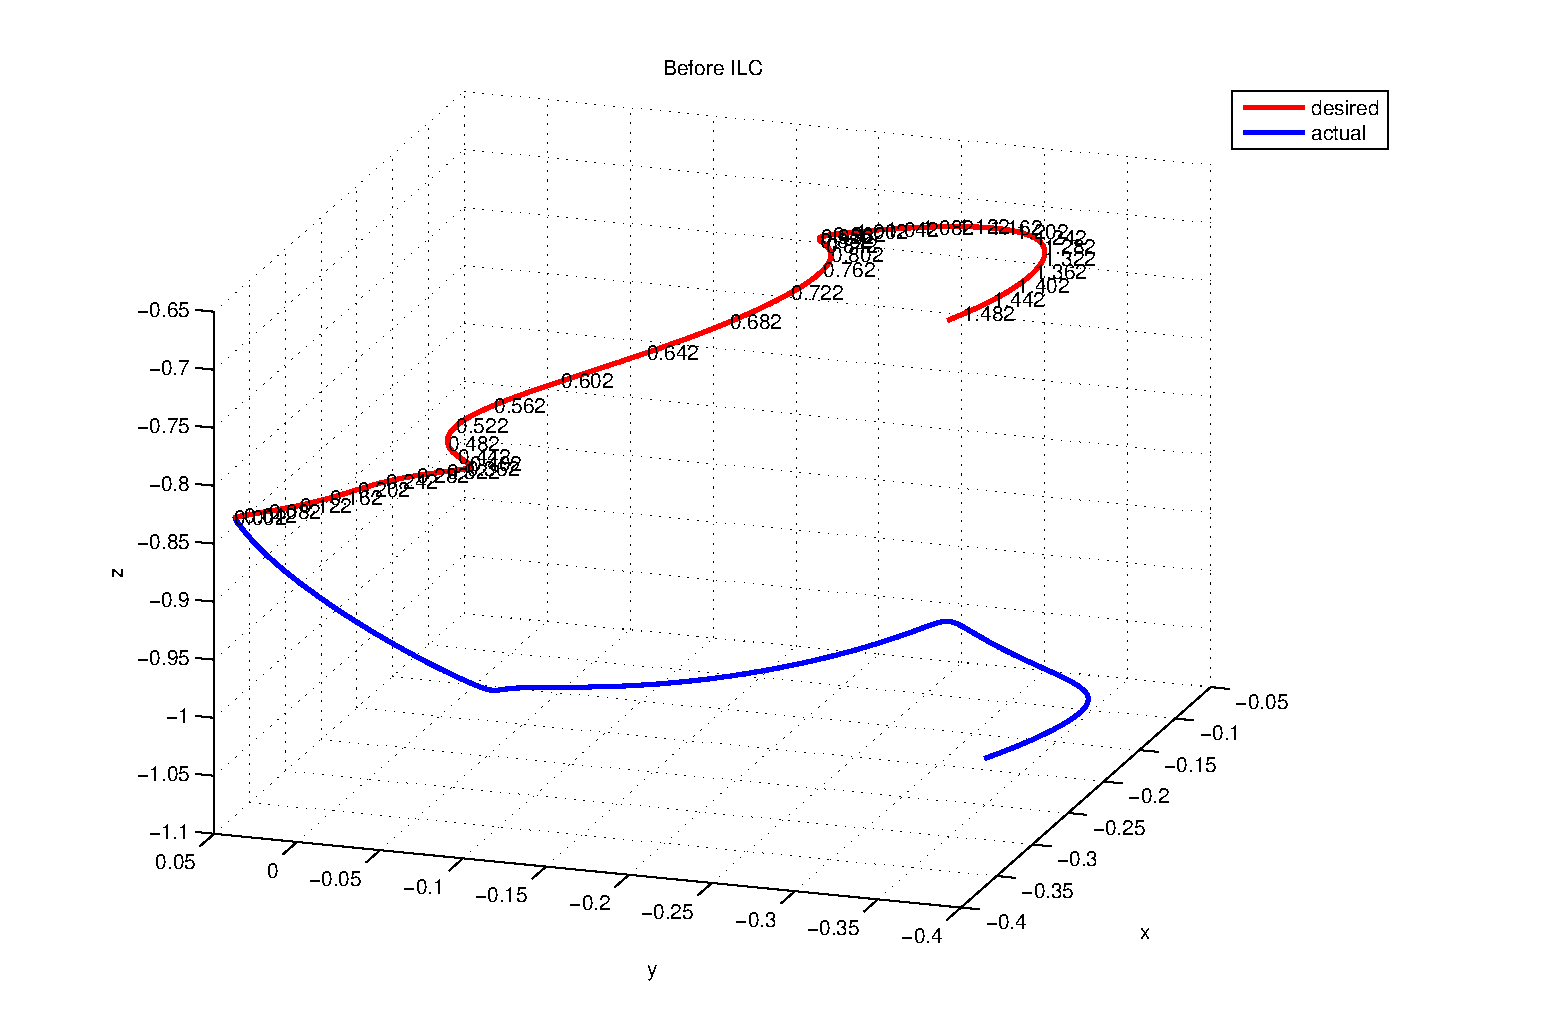
\includegraphics[width=\linewidth, height=0.15\textheight]{beforeILC.eps}
        \caption{(a)}
        \label{fig1}
    \end{minipage}%
    \begin{minipage}{.25\textwidth}
        \centering
        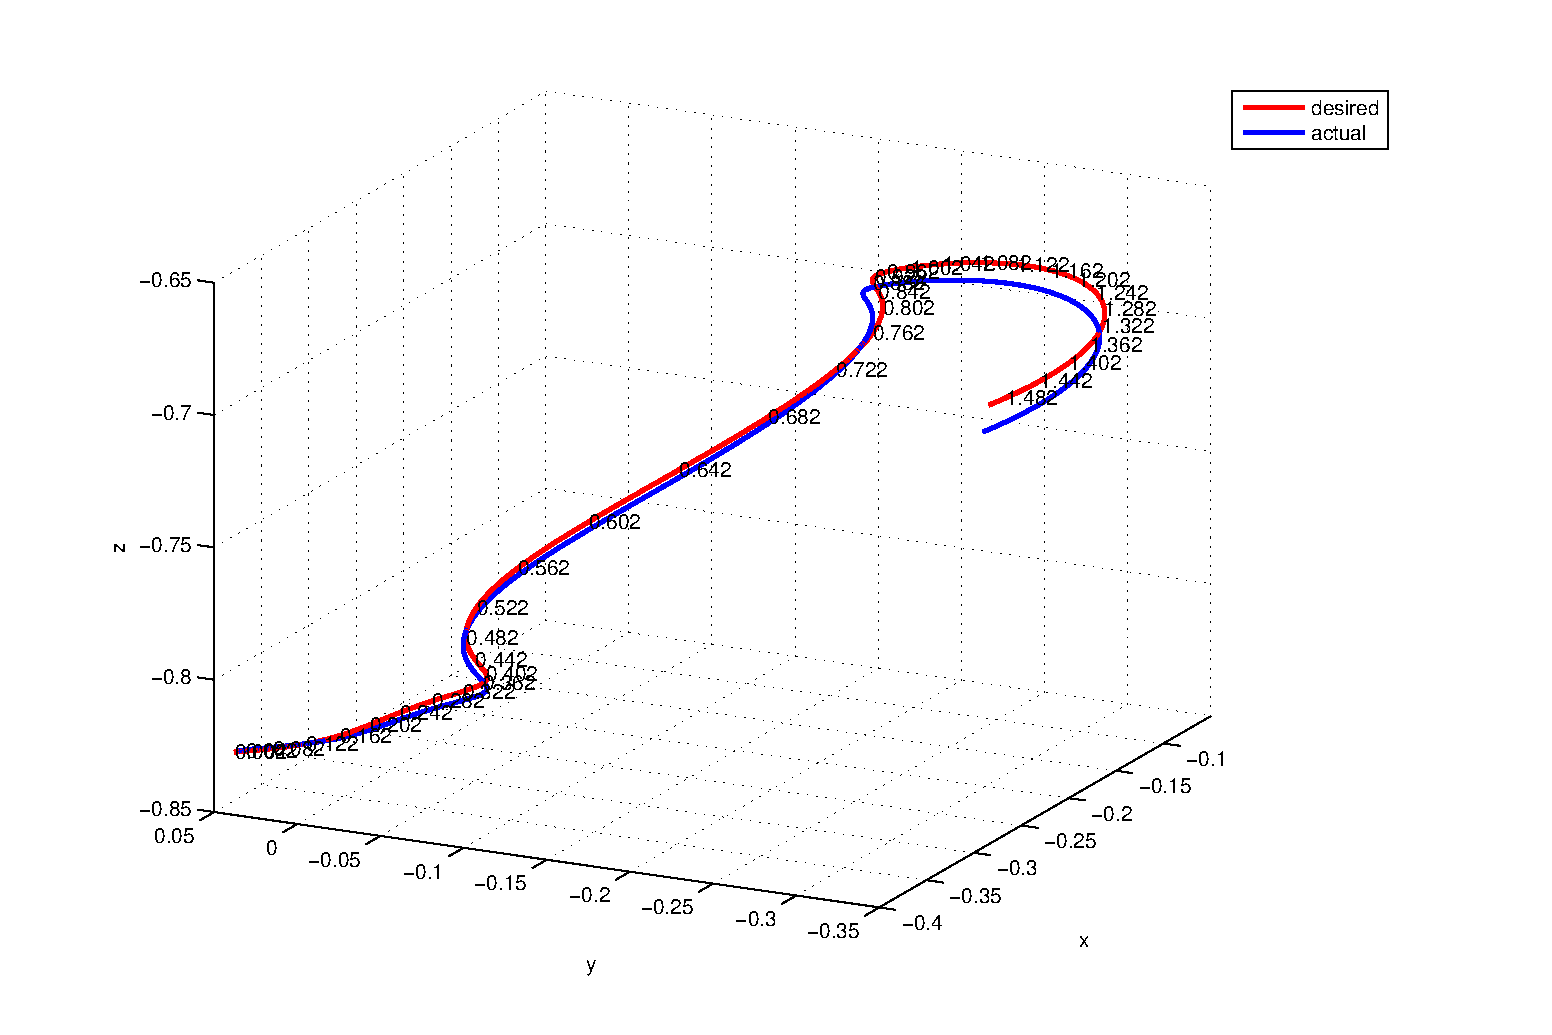
\includegraphics[width=\linewidth, height=0.15\textheight]{afterILCPseudoInv.eps}
        \caption{(b)}
        \label{fig2}
    \end{minipage}
    \begin{minipage}{.25\textwidth}
        \centering
        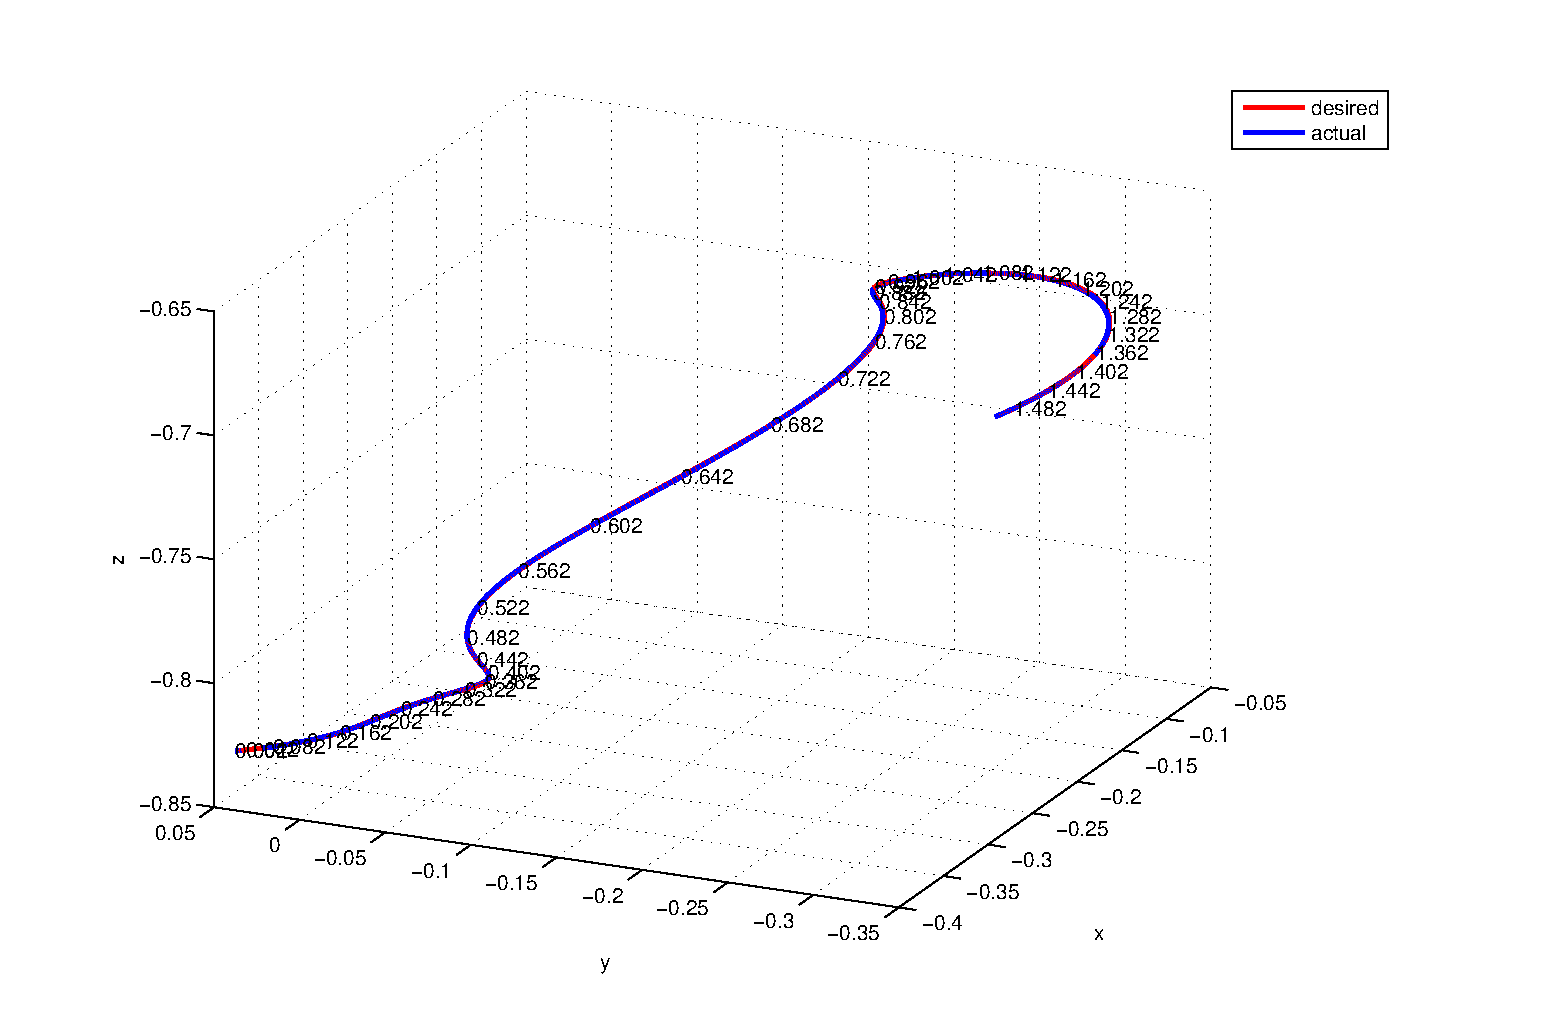
\includegraphics[width=\linewidth, height=0.15\textheight]{afterILCTLS.eps}
        \caption{(c)}
        \label{fig3}
    \end{minipage}
    \caption{Results showing the performance of trajectory tracking, before and after applying ILC (10 iterations). Reference trajectory is shown in red. Initially, in Figure~\ref{fig1}, tracking performance is poor. Final performances of pseudoinverse-based ILC and TLS-based ILC after learning are shown in Figures~\ref{fig2} and \ref{fig3} respectively. ILC with truncated pseudoinverse cannot approach the trajectory very well, and after 8 iterations starts to slowly diverge. ILC with truncated total least squares on the other hand approaches the trajectory very well, and shows excellent tracking performance that is also stable.}
\label{FigureILC}
\end{figure}

In the simulation results shown in Figure~\ref{FigureILC}, we consider a striking trajectory shown in red. Such ball-hitting trajectories in table tennis are generally composed of three parts: a preparatory phase, a hitting phase, and a relaxation phase. In the preparatory phase, the arm generally accelerates and picks up speed necessary to transfer the right momentum to the ball, intercepted in the hitting phase. The relaxation phase generally decelerates the arm and readies it for the next hitting task. 

ILC with pseudoinverse cannot approach trajectory very well, and after 8 iterations starts to slowly diverge. ILC with TLS on the other hand approaches the trajectory very well, and shows excellent tracking performance. For both methods, to be fair, we used the same truncation parameter, $\epsilon = 0.05$. This enables the pseudoinverse-based ILC to be more stable, i.e. without it ILC can show dangerous oscillations around some trajectories. However, even with truncation the pseudoinverse relies on the exactness of the model, whereas $\alg$ is inherently \emph{agnostic} to its accuracy. 

In practice we find that an additional adjustment in the form of \emph{current-iteration} ILC (\emph{CI-ILC}) 
%
\begin{equation}
\begin{aligned}
\sysInput_{k+1} &= \sysInput_k - \vec{K}_{LQR}\error_{k},\\
\end{aligned}
\label{fbILC}
\end{equation}
%
\noindent where we add the feedback from the previous iteration to the feedforward commands in the next iteration makes learning more robust. We add this current-iteration compensation to both methods in the results shown. 


\subsection{Applications in Robotic Table Tennis}

We performed the real robot experiments with a seven degree of freedom (DoF) torque-controlled custom made Barrett WAM arm capable of high speeds and accelerations.
%\section{CONCLUSION}\label{end}

% shall we put inv. dynamics eq here?
The cost functional to be minimized considers the accelerations as the quantity to be minimized. It assumes that the feedback linearization of the robot is perfect, that is the inverse dynamics model for the robot is exact. Whenever the cancellation is imperfect due to inaccurate robot control, execution error will prevent the robot from achieving the desired trajectories. Execution errors will be considered in future work.

\section{INTRODUCTION}

The opponent's court in table tennis, the net and other environmental restrictions such as walls together define a natural \emph{stability region} that is intrinsic to the game: the table tennis playing robot implementing our favorite reinforcement learning and control algorithm will lose a point if they cannot land the ball on the other side of the table. Taken in a wider sense, this stability region is a result of the redundancy in task-specification, and should be exploited as much as possible in all robotic tasks. 
% $\court$

An aspect in table tennis that strengthens this point is the uncertainty in ball estimation. As a result of limitations in the sensing hardware as well as in our simple physical models that neglect certain dynamics, the ball cannot be estimated or predicted perfectly within the workspace of the robot. In an ideal world where this could be done, exploitation of task-redundancy could indeed be relegated to a higher-level strategy, as is often done in previous works in table tennis~\cite{Muelling13}. However, whenever there is ball uncertainty, being aware and taking advantage of the stability region is critical and directly contributes to generating successful playing styles.
%  It is difficult to estimate the center of mass of the ball from image data. Small errors in position can accumulate to much larger errors in velocity estimates. Moreover, the ball is very light and some effects such as spin cannot be predicted precisely even with sophisticated modelling.

% But nobody should blame them if they land the ball precisely on a target point but only within a certain region of it: they do not have to! Even humans with very agile striking capabilities are not able to return the ball to a precise location.
% mention human studies in this aspect

In this paper, we incorporate probabilistic modeling for robust trajectory generation and come up with a new performance criterion in table tennis that exploits the game's natural stability criterion. The cost functional that we try to minimize is not \emph{certainty-equivalent} and naturally leads to \emph{cautious} strategies. Moreover it is particularly suitable for employing adaptive strategies as the robot gets more data and refines its internal models of the environment. 

Our approach involves intensive modeling of task-relevant quantities from data, e.g. ball flight, bounce models and ball-racket contact modeling. The last one especially can be hard to train from missing data. However, we keep the uncertainty of all of our models and use them also in our decision-making process. This cautious design is an asset that differentiates our approach from previous approaches (e.g. \cite{Matsushima05}, \cite{Muelling13}) that are less robust to modeling and estimation uncertainty.
% from missing data and can even be misleading when given example ball trajectories with high spin.

To summarize our reasons for introducing uncertainty and probabilistic modeling to trajectory generation in table tennis: \textit{i)} Table tennis balls are very light and cannot be estimated or predicted precisely. \textit{ii)} Racket-ball interaction is generally not known well and the elasticity of the momentum exchange differentiates it from the mirror laws used in the literature so far. \textit{iii)} The set of allowed landing point specifications in the opponent's side can be incorporated to design robust algorithms that return the ball with a higher probability, when under the influence of various effects mentioned in \textit{(i)} and \textit{(ii)}. See figure~\ref{mainIdea} for an illustration.% ref needed obviously 
% velocity dependent coefficient of restitution

% The choice of the the desired landing point of the ball on the opponent's court is generally left to a higher level strategy or policy of the robot. However in this paper we argue that landing the ball successfully on the opponent's court is the \emph{fundamental goal} in table tennis. Therefore policies or the strategies involved in striking movement generation should be combined in one unitary whole.

\begin{figure}[t!]
\center
\includegraphics[scale=0.4]{robot1.png}			
\caption{Robotic table tennis setup with four cameras tracking the ball at 60 Hz. In order to return the ball to the opponent's court, we need to consider the uncertainty in ball estimation as well as in our ball-racket contact model. Introducing uncertainty into planning and a more cautious generation of striking trajectories will allow us to return the ball with a higher probability.}
\label{robot}
\end{figure}
% REPLACE PHOTO WITH ANOTHER ONE INCLUDING CAMERAS

In the rest of this paper, we elaborate on this notion of robustness, giving more examples and the necessary intuition where needed. In Section~\ref{relatedWork} we introduce previous work on table tennis and other relevant trajectory generation frameworks. In Section~\ref{method} we formalize robot trajectory generation as a specific optimal control problem and incorporate probabilistic modeling within this framework. We do not know of any closed-form solutions even in simplified cases. In Section~\ref{alg} we discuss a Monte-Carlo based rejection sampling approach for optimizing the previously introduced cost functional. In Section~\ref{results} we evaluate the performance of this approach and compare it with previous inverse kinematics (IK) approaches. When the inverse dynamics models are not known well for the robot, robustness with respect to trajectory \emph{execution} must be additionally considered. In the final section~\ref{end} we discuss several promising extensions in this regard. %VHP-based

\begin{figure}[t!]
\centering
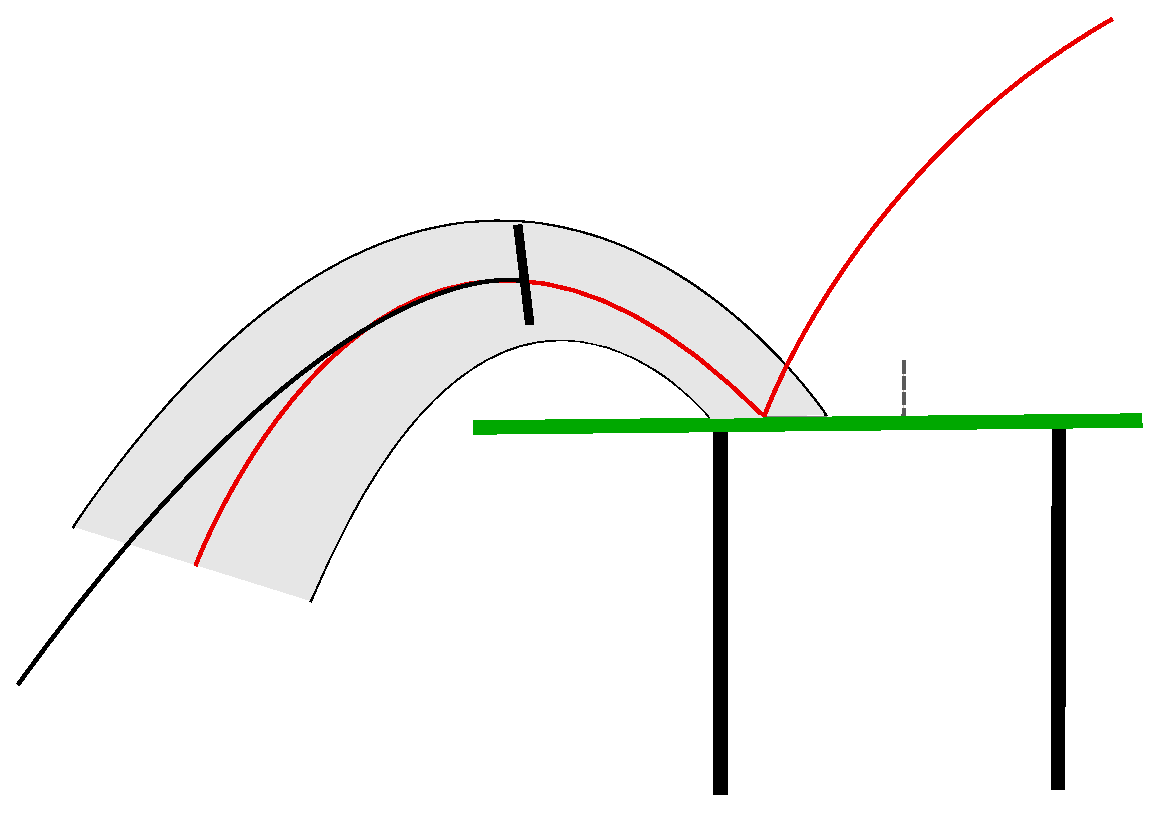
\includegraphics[scale=0.4]{drawing.eps}			
\caption{Illustrating the main idea behind this paper: from the ball's point of view, a racket trajectory in table tennis has a certain probability of hitting the ball and a significantly smaller probability of landing it (legally) on the opponents court. From the racket's point of view, the ball motion is a certain stochastic process and it should be intercepted such that the marginal probability distribution at hitting time is transformed at landing time to a desired marginal distribution. Racket trajectory and the mean of the ball trajectory are shown in black and red, respectively. }
\label{mainIdea}
\end{figure}

\section{RELATED WORK}\label{relatedWork}

% % % % Striking Movement Generation in Humans % % % % %
% speed-accuracy trade-off [Woodworth 1899, Fitts 1954]
% variability [Todorov and Jordan, 2002]
% goal-directed corrections [Elliott et al.]
% biomechanical redundancy [Bernstein, 1967]
% cost functions from optimal control [ Bryson and Ho, 1975; Hogan, 1984; Harris and Wolpert, 1998; Todorov and Jordan, 2002]
% motor program [Henry and Rogers, 1960; Keele, 19658; Schmidt, 1975; Schmidt and Wrisber, 2000, Schmidt, 2003]
% related: operational timing hypothesis [Tyldesley and Whiting, 1975]
% tau hypothesis to account for the time-to-contact: tau is specified as the relative inverse rate of dilation of the object image [Lee and Young, 1985; evidence for it: Bootsma and van Wieringen, 1988]
% stroke timing independent of ball speed [Hubbard and Seng, 1954] 
% error tolerance [Dagmar Sternad, Hermann Mueller, 2011]
% funnel-like control with fixed spatio-temporal bandwidth [Bootsma and Peper, 1992; Williams and Starkes, 2002]

% % % % Cost functions for movement generation % % % %
% cost of the movement includes - jerk, (metabolic) energy [Bryson and Ho, 1975]
% relationships found in reaching and pointing movements do not hold in striking sports [Bootsma and van Wieringen, 1990]
% energy optimality [Alexander, 1997; Kuo, 2005]
% Comfort of the posture, i.e. cost is induced by proximity to a fixed comfort posture in joint-space. 
% We believe that a new performance criterion in robotic table tennis is needed to explain the robust trajectory generation frequently observed in humans, and in order to compete with them. 

% robust movement generation
% robust algorithms that can compensate for low quality hardware and uncertainty in ball estimation

% hitting stage lasts approximately 80 ms in expert humans [only find a robust hitting trajectory]

% make sure to cite Marco Campi's scenario approach in robust control
% cite Stochastic Minimum Principle papers

\section{METHOD}\label{method}

In table tennis, one needs to determine when, where and how to intercept the incoming ball trajectory. So far, most of the algorithms for robotic table tennis \cite{Muelling13} calculate the intersection point of an estimated ball trajectory with a Virtual Hitting Plane (VHP) to determine the space and time coordinates of the hitting point. To estimate the trajectory of the ball, we require as data, a stream of estimates of ball position. We terminate the estimation process after a bounce event has been detected with high probability. 
% do we really need a fixed event such as bounce to terminate the estimation process?
%It is possible to eliminate this termination event altogether and vary the robot trajectory launch times based on ball estimates.

For safety reasons, VHP algorithms need to specify a minimum hitting time $T_{\textrm{min}}$ in addition to the coordinates of the hitting plane. When the ball is coming very fast towards the VHP, any calculated trajectory of duration below the minimum time will simply not be executed. This will prevent high accelerations and any risk of damage to the robot. However the determination of this minimum hitting time can be arbitrary, and the algorithms involving a VHP can lead to unnecessarily strict or restrictive strokes.
% impact time, ball position and velocity
% time to contact

After accounting for the net and any other environmental constraints such as walls, the stability region of table tennis reduces to the Cartesian coordinates of the table $\court$ as a rectangular region with a fixed vertical distance $z_{\court}$ from origin. Any algorithm that can return the ball to this fixed region can be said to be \emph{stable}.


\subsection{Learning Models From Data}

% air resistance scale factor C 
% $\ballFull = (\ball^{\mathrm{T}},\dot{\ball^{\mathrm{T}}})^{\mathrm{T}}$
We require three models for the trajectory generation process and acquire them (iteratively) from raw ball data. The ballistic \emph{flight model} $\ddot{\ball} = \ballDynamics(\dot{\ball})$ is a nonlinear model that describes the ball dynamics and generally involves air drag $\drag$ and gravity $\gravity$. The \emph{rebound model} $\dot{\ball}_{\mathrm{out}} = \bounce\dot{\ball}_{\mathrm{in}}$ is a discrete event with diagonal entries of $\bounce$ as coefficients $\epsilon = [\epsilon_{x}, \epsilon_{y}, -\epsilon_{z}]$. The coefficient of restitution $\epsilon_{z}$ accounts for the reflection of velocity in the vertical direction $z$ and $\epsilon_{x}, \epsilon_{y}$ are the coefficients of friction along the planar $x,y$ directions.
% incoming ball trajectory: as Gaussians indexed with time [e.g. Kalman filter should give us this information with prediction. Parameters/model of a Kalman filter could be fit using ball data (when fitting, innovation of the KF should be minimized as to consist mostly of white noise)]

% A probabilistic model describing the interaction model: outputs a probability distribution of outgoing ball states parameterized (or indexed) by t, e.g. b_t \approx N(\mu_b_out(t), \sigma_b_out(t))

% build a forward/inverse interaction model probabilistically
The last model to train from data is the \emph{ball-racket contact model} $\ \dot{\ball}_{\mathrm{out}} = \contact(\dot{\ball}_{\mathrm{in}},\dot{\racket},\orient)$. This model is significantly harder to train from the previous models, as it requires ball-racket interaction data and it is difficult to get reliable ball estimates around hitting time. We need to instead rely on smoothing using the trained flight model and the samples before and after hitting. In previous works, the outgoing velocity of the ball is calculated using a \emph{mirror law}: $o_{\parallel} - v = \epsilon_{R} (-i_{\parallel} + v)$ with $v$ the speed of the racket along its normal and $\epsilon_{R}$ the coefficient of restitution on the racket. $o_{\parallel}$ and $i_{\parallel}$ are the outgoing and incoming ball velocities along the racket, respectively. This model assumes an elastic momentum exchange and it is quite inaccurate, especially at high ball velocities.
% is this true? is the parallel o and i definitions correct?

The accuracy of these models all depend on each other and for this reason, we train the parameters of these models with the Expectation-Maximization (EM) algorithm. Effects of angular velocity, or in other words spin, are not accounted for in these models. During test time when running these trained models online, an Extended Kalman Filter (EKF) or any regression method to estimate initial ball position and velocity can use these models to perform prediction and update steps.

\subsection{Predicting with Probabilistic Modeling}

% density or distribution
Using an EKF for our nonlinear model $\ballDynamics$ generates at each time instant $t$ a probability distribution $p_t(x,y,z|t)$ of incoming ball states parameterized by time, e.g. $\ball_t \sim \mathcal{N}(\vec{\mu}_{\textrm{in}}(t),\vec{\Sigma}_{\textrm{in}}(t))$. 

% % % EXT. KALMAN FILTER EQUATIONS HERE % % %

Formally this is a stochastic process, and for the Kalman Filter with a noisy process model, a Brownian motion. However we set the process covariance to zero during prediction, as the sample paths of the exponential kernel used in the Kalman Filter framework are very rough, i.e. almost surely not differentiable.

% Interaction probabilities (ball touching the racket)
Prediction continues after a possible interaction with the racket trajectory. If the ball touches the racket, i.e. if the surface of the ball is located inside the radius $\racketRadius = 8$ cm of the racket plane, ball incoming velocities will be transformed according to the trained contact model. Otherwise the ball with continue its previous projectile-like motion. Prediction is stopped when the ball hits the table plane with negative velocity in the $z$ direction.

\subsection{Optimal Control for Trajectory Generation}

From a set point of view, for every point on the predicted ball trajectory, there is a range of admissible outgoing ball velocities that the racket can impart. This set is constricted by the geometry of the table and the demands of the game: the ball has to avoid the net and the walls and should land on the opponents court. Probabilistically speaking, the landing point could be any distribution with compact support over the table, e.g. a uniform distribution $x_{\textrm{land}}, y_{\textrm{land}} \sim \mathcal{U}(\court) = \mathcal{U}(x_{a},x_{b})\mathcal{U}(y_{a},y_{b})$ or a truncated normal distribution. The limiting values $x_{a},x_{b},y_{a},y_{b}$ are obtained from the rectangular geometry of the opponent's court.
%

Our optimization criterion of choice is to find the racket trajectory that minimizes the Kullback-Leibler (KL) divergence $\textrm{KL}(p\|q) = \int_{\court}p(x,y)\log(\frac{p(x,y)}{q(x,y)})\textrm{d}x\textrm{d}y$ of $p(x,y|z_{\court},\dot{z} < 0) = \int_{\hitTime = 0}^{\infty} p_{\hitTime}(x,y|z_{\court},\dot{z} < 0,\hitTime)\hitDist \textrm{d}\hitTime$ with a desired distribution imposed by the robotic player. $p(x,y|z_{\court},\dot{z} < 0)$ is the marginal distribution over time of the ball process $p_t(\cdot)$. Other more agnostic optimization criteria could also be formulated to minimize the racket trajectory sensitivity to perturbations in the ball trajectory. However these would not take advantage of the uncertainty quantification of the ball trajectory, in our case supplied by EKF.

% what about maximizing the probability of landing, regardless of any specified distribution?
% is this true?
Any specified distribution $q(\cdot)$ of compact support $\court$ will indirectly maximize the probability of landing on the table, $\prob(\textrm{land}) = \int_{0}^{\infty}\landDist\textrm{d}\landTime$. Here $\landTime$ is a \emph{hitting time} random variable of the set $\court$. In addition, for maximal unpredictability, the robot player can choose the uniform distribution over the table as a desired distribution. In this case the optimization reduces to maximizing the entropy of the landing distribution on the table. 

For safety and efficiency, we would prefer trajectories with minimal acceleration or jerk, the derivative of acceleration. Combining the minimal acceleration criterion with the KL-divergence we get
%
\begin{align}
\min \int\limits_{0}^{T}\ddot{\joint}(t) + \textrm{KL}(p(x,y|z_{\court},\dot{z}<0)|\mathcal{U}(\court)),
\label{costFnc1}
\end{align}
%
where the marginal distribution $p(x,y|z_{\court},\dot{z}<0)$ of the ball process can be written as
%
% should we give also the probability of landing here?
\begin{align}
p(x,y|z_{\court},\dot{z}<0) &= \int_{\landTime = 0}^{\infty} p_{\landTime}(x,y|z_{\court},\dot{z}<0,\landTime)\hitDist \textrm{d}\landTime \label{marginalDistr1}, \\
p_{\landTime}(x,y|z_{\court},\dot{z}<0,\landTime) &= \frac{ \int_{\dot{z}=-\infty}^{0}\int_{\dot{x},\dot{y}}p_{\landTime}(x,y,z_{\court},\dot{x},\dot{y},\dot{z}|\landTime)}{p(z_{\court},\dot{z}<0)}.
\label{marginalDistr2}
\end{align}
%
The marginal distribution over $x,y$ velocities appearing in the numerator of \eqref{marginalDistr2} is
\begin{align}
& p_{\landTime}(x,y,z,\dot{z}|\landTime) = \int_{\hitTime = 0}^{T} \int_{\dot{x},\dot{y}}  p_{\landTime}(x,y,z,\dot{x},\dot{y},\dot{z}|\ball_{\textrm{out}},\dot{\ball}_{\textrm{out}},\landTime) \times \\
& p(\dot{\ball}_{\textrm{out}}|\dot{\ball}_{\textrm{in}},\dot{\racket}(\hitTime),\orient(\hitTime),\hitTime)p(\ball_{\textrm{out}}|\ball_{\textrm{in}},\racket(\hitTime),\orient(\hitTime),\hitTime)\hitDist\textrm{d}\hitTime.
\label{fullDistr}
\end{align}
%
where $\hitTime$ is the hitting time random variable corresponding to the time of ball-racket contact, $\prob(\textrm{hit}) = \int_{0}^{T}\hitDist\textrm{d}\hitTime$. In \eqref{fullDistr} the probability densities are obtained using the trained models, i.e. the flight model and the ball-racket contact model. 

By formulating \eqref{costFnc1} in joint space, we find the joint trajectory $\joint(t)$ that provides a suitable trade-off between minimum joint accelerations $\ddot{\joint}(t)$ and maximum probability of landing $\prob(\textrm{land})$. Using direct kinematics we can obtain the desired racket trajectory and orientations, i.e. $[\racket(t),\orient(t)] = \kin(\joint(t))$.




% Output
% 
% The mapping r_t \approx N(\mu_racket_center(t),\sigma_racket_center(t))) as racket reference trajectory that maximizes the probability of landing on the opponents court, or minimizing KL-divergence between outgoing ball states distribution and admissable/desired velocities [e.g. uniform distribution of velocities]

% Control: imposing transversality conditions when ball is on a curve p_b(t) or a set with some measure p_b [constant hamiltonian on this set?] we get a probability distribution of admissable end effector configurations
%
%
% Probability of interaction occurring: b(t) for the ball must lie in r(t) + \gamma o_\parallel(t), where r(t) is the racket centre trajectory, \gamma is less than the radius of the racket, and o_\parallel(t) is any direction perpendicular to the normal (i.e. orientation) of the racket.
%

% Refer to article for the simplest case when diving two Gaussians with nonzero mean.
We do not know of any way to compute the ball landing distribution in closed form, as a function of racket positions and orientations. However, the outgoing ball trajectory is an integral over the previous incoming ball distribution using the ball-racket contact model. Any sampling based approach (e.g. rejection sampling) may be used to simulate then the outgoing ball trajectory and approximate the resulting landing distribution. 


\section{ALGORITHM}\label{alg}

\section{EXPERIMENTS}\label{results}

% % % CHANGE THE WRITING HERE !!! OTHERWISE ITS THE SAME AS PREVIOUS ARTICLE

% % % % Table Tennis Setup % % % %
For the robotic table tennis task we are using a seven degree of freedom (DoF) torque-controlled custom made Barrett WAM arm capable of high speeds and accelerations. A standard size racket (16 cm diameter) is mounted on the end-effector of the arm as can be seen in Figure~\ref{robot}. A vision system consisting of four cameras hanging from the ceiling around each corner of the table is used for tracking the ball \cite{Lampert12}. The orange ball is tracked visually with a sampling rate of 60 Hz and filtered with an EKF that accounts for some of the bouncing behavior of the ball and air drag effects. The table and the tennis balls are in accordance with the International Table Tennis Federation (ITTF) rules.
%
A ball launcher (see Figure~\ref{robot}) is available to throw balls accurately to a fixed position in Cartesian space to the forehand of the robot. The incoming ball arrives with low-variability in desired positions and higher-variability in ball velocities. The whole area to be covered amounts to about 1 m$^2$ circular region surrounding the initial forehand posture of the robot. This allows us to avoid the singularities of the robot. Any ball that appears outside of this circular \emph{feasible} region will not be hit.
%
After the visual system predicts a ball trajectory that coincides with the feasible region in Cartesian space, the motion planning system has to come up with a trajectory that specifies how, where and when to intercept the incoming ball. 
%Desired Cartesian position, velocity and orientations of the racket translate in joint space to a specification of 14 parameters: 7 joint angles and 7 joint velocities of the robot arm. Along with the desired hitting time (or the time until impact), these 15 parameters are used to train 7 joint space trajectories that correspond to the desired reference trajectory in Cartesian space.
%
In runtime, in order to generate feasible reference trajectories that account for the variations in incoming ball position and velocities, we run the robust trajectory generation framework $\alg$. We start these joint reference trajectories from the initial posture of the robot provided by the sensors.
% From Katharina's paper:
%the position, velocity and orientation of the racket can be computed analytically based on the state of the system and the target on the opponents court.
%These task space parameters can also be converted into joint space parameters using inverse kinematics

Due to the limitations of our setup, our robot is fixed to the ceiling. Hence we expect that the balls that hit the frontal areas of the robots table will not be hit. The table can be brought closer to the robot to overcome this limitation: however then the trajectory generation problem will be subsequently harder, and the hard constraint of hitting the table becomes more problematic to avoid.

% vision system operates in a semi-structured and human-inhabited environment
% Finite State Automaton: four stages: awaiting stage, preparation, hitting and finishing stage

\section{CONCLUSION}\label{end}

% stochastic optimal control
We see the probabilistic extensions of Pontryagin's minimum principle as a very fruitful direction for robotics in general in the upcoming years, as robots start taking decisions in complex, demanding tasks. The robot trajectories to be generated can also taken to be probabilistic, leading to an optimization framework that considers the interaction between two probability distributions. We consider the probabilistic movement primitives~\cite{Paraschos13} to be a step in the right direction.

% reinforcement learning to modify trajectories

The cost functional to be minimized considers the accelerations as the quantity to be minimized. It assumes that the feedback linearization of the robot is perfect, that is the inverse dynamics model for the robot is exact. Whenever the cancellation is imperfect due to inaccurate robot control, execution error will prevent the robot from achieving the desired trajectories. Execution errors are not taken into consideration within this framework. 

A natural reward signal to use for reinforcement learning is to look at the set-distance of the landing point from the opponents court. This reward can be used to modify the generated trajectories and learn to compensate for the execution errors. Another promising approach is Iterative Learning Control (ILC), see for example \cite{Bristow06}, \cite{Longman2000}, \cite{Koc15}. ILC is a more efficient learning approach that generally makes more assumptions. Generalizing ILC to different trajectories generated by $\alg$, we hope to increase the performance of our robot further. 

\bibliographystyle{plain}
%\bibliographystyle{./IEEEtran}
%\bibliography{./IEEEabrv,./iros2015Ref}
\bibliography{./ttRef}

\end{document}
